\documentclass[12pt,border=4pt,multi]{article} % \documentclass[tikz,border=4pt,multi]{article}
\usepackage{lingmacros}
\usepackage{tree-dvips}
\usepackage{amssymb} % for mathbb{}
\usepackage[dvipsnames]{xcolor}
\usepackage{forest}
\usepackage{amsmath} % for matrices
\usepackage{xeCJK}
\usepackage{tikz}
\usepackage[arrowdel]{physics}
\usepackage{graphicx}
\usepackage{wrapfig}
\usepackage{listings}
\usepackage{pgfplots, pgfplotstable}
\usepackage{diagbox} % diagonal line in cell
\usepackage[usestackEOL]{stackengine}
\usepackage{multirow}
\graphicspath{{./img}} % specify the graphics path to be relative to the main .tex file, denoting the main .tex file directory as ./
\definecolor{orchid}{rgb}{0.7, 0.4, 1.1}

\begin{document}

\section*{Xi Liu, xl3504, final}
\begin{verbatim}
 You may use the textbook, slides, and any notes you have.
But you may not use the internet. 
 You may NOT use communication tools 
to collaborate with other humans.
 Do not try to search for answers
on the internet. It will show in your answer, and you will 
earn an immediate grade of 0. 
 Anyone found sharing answers 
or communicating with another student
during the exam period will earn an immediate grade of 0. 
 "I understand the ground rules and agree to abide by them. 
I will not share answers or assist another student during this exam,
nor will I seek assistance from another 
student or attempt to view their answers.” 
\end{verbatim}
\newpage
\noindent
Problem 1\\
a\\
based on Amdahl's law:\\
let $F$ be the fraction of sequential part of the program\\
let $S$ be the speedup\\
let $p$ be the number of cores available to use\\
$F = 1 - 0.9 = 0.1$\\
$p = 10$\\
\begin{align*}
S &= \frac{1}{(1 - F)/p + F}\\
&= \frac{1}{(1 - 0.1)/10 + 0.1}\\
&\approx \boxed{5.3}\\
\end{align*}
\newpage 
\noindent
b\\
let $F$ be the fraction of sequential part of the program
\begin{align*}
\text{Amdahl's law:}\\
S &= \frac{1}{(1 - F)/p + F}\\
\text{substitute } S = 2, \quad p = 4\\
2 &= \frac{1}{(1 - F)/4 + F}\\
2 &= \frac{1}{1/4 - F/4 + 4F/4}\\
2 &= \frac{1}{1/4 + 3F/4}\\
2 &= \frac{1}{(1 + 3F)/4}\\
2 &= \frac{4}{1 + 3F}\\
1 + 3F &= \frac{4}{2} = 2\\
3F &= 1\\
F &= \boxed{\frac{1}{3}}\\
\end{align*}
\newpage
\noindent
c\\
reason 1: directory-based cache coherence uses the directory data structure to store each cache line's status. additional storage is used for the directory. if a variable is updated, there is additional time needed to consult the directory, and more time required when cores that store a variable need to be signaled if a cache variable is updated\\ 
reason 2: snooping cache coherence needs information regarding cache line update to be broadcast across all cores, which is slow and creates traffic, extra time might be needed to transfer the data through the interconnect\\
reason 3: false sharing due to cache coherence protocol. CPU caches operate on cache lines but not variables since CPU caches are hardware implementations. suppose that in a loop, we need to use an array to store the results of some computations, partition the work of the loop iterations to be executed by multiple cores. the data of the array is stored in 1 cache line. then each read or write to 1 element of the array invalidates the entire cache line, which leads to more main memory accesses\\
reason 4: invalidation in cache protocol can result in additional cache misses\\
\newpage
\noindent
Problem 2\\
a\\
option 1:
\begin{lstlisting}
MPI_Allreduce(A, B, 4, MPI_INT, MPI_BAND, NEWCOMM);
\end{lstlisting}
\leavevmode
\\
\\
option 2 (conditional, if assumption is satisfied):\\
the 1 line function call to broadcast to send the data to all other processes is
\begin{lstlisting}
MPI_Bcast(B, 4, MPI_INT, 0, NEWCOMM);
\end{lstlisting}
which required the assumption that the data $\{0, 0, 8, 8\}$ is copied to process 0's allocated storage pointed to by B before the function call\\
\leavevmode
\\
\\
\\
\\
b\\
minimum number of communicators is 2 if MPI\_Comm\_free() or some other functions are not used to destroy NEWCOMM, then communicators NEWCOMM and MPI\_COMM\_WORLD are there\\
minimum number of communicators is 1 if MPI\_Comm\_free() or some other functions are used to destroy NEWCOMM, then the only communicator left is MPI\_COMM\_WORLD\\
\\
\\
\\
\\
c\\
yes, there is 2 * 16 = 32 cores available, if each of the 4 processes make 8 threads, then 4 * 8 = 32 cores can be used at the same time\\
\newpage
\noindent
Problem 3\\
a\\
need to use #pragma omp master when the structured code block need to be executed by the master thread (or thread 0) only but not other thread, #pragma omp single only guarantees the structured code block is executed by only 1 of the threads in the team but #pragma omp single cannot guarantee which thread execute the structured code block\\ 
\\
\\
\\
\\
b\\
parallelize the inner loop\\
reason 1: no dependency between rows, so each row should be parallelized, so parallelize the inner loop that controls the row index $j$. there is only dependency among columns or elements within the same row since $v$ is accessed through $v[j][i-1], v[j][i],$ and $v[j][i+1]$, which means the only the second or column dimension changes due to $i$\\
reason 2: cache friendliness and spatial locality: since the inner loop increments $j$, and $v$ is accessed using $v[j][i]$, which means in each of the iterations of the inner for loop, $v$ is accessed through $v[0][i],\; v[1][i],\; v[2][i],\;...,\; v[n - 1][i]$, since $v$ is a 2 dimensional data structure and 2 dimensional arrays are stored linearly (1 row after another) in C language, accessing $v$ in row-major order ($v[i][0],\; v[i][1],\; v[i][2],\;...,\; v[i][n - 1]$) is more cache friendly and has more spatial locality than accessing $v$ in column-major order ($v[0][j],\; v[1][j],\; v[2][j],\;...,\; v[n - 1][j]$). \\
\newpage
\noindent
c
\begin{figure}[h!]
	\centering
	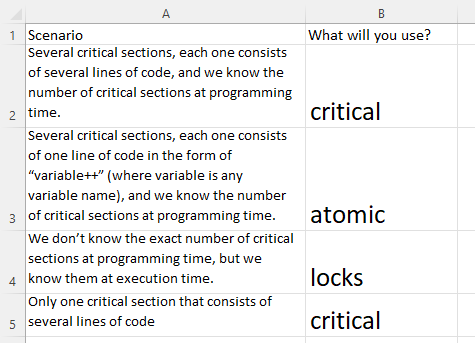
\includegraphics[width=\textwidth, height=0.9\textwidth]{3c} %img size
\end{figure}\\
\newpage
\noindent 
Problem 4\\
for this question, assume the problem intends to say “printf(“\%d", x)" instead of “printf(“x”)" within the else code block of the printing() function\\ 
\\
a\\
a. not possible, b. not possible, c. not possible, d. not possible, e. not possible, f. not possible\\
\\
\\
\\
\\
b\\
no change\\ 
answers are still\\
a. not possible, b. not possible, c. not possible, d. not possible, e. not possible, f. not possible\\
\_\_shared\_\_ int x = 7 is a compiler error since initializer is not allowed for \_\_shared\_\_ variable, this error can be removed if removed \_\_shared\_\_ keyword. however, everything is still not possible since there is a barrier imposed as the result of having a warp for each block, so all the threads in each block must execute in a lockstep, this means “77” should be printed consecutively (printf("\%d", x) from 2 threads in block 0), “22” should be printed consecutively (printf("\%d", blockIdx.x) from 2 threads in block 2), “11” should be printed consecutively (printf("\%d", blockIdx.x) from 2 threads in block 1)\\
\\
\\
\\
\\
c\\
no change\\
answers are still\\
a. not possible, b. not possible, c. not possible, d. not possible, e. not possible, f. not possible\\
\_\_syncthreads() has no effect since each block has only 2 threads, which is less than 32 threads (warp size), so each block has 1 warp, all instructions in the warp execute in a lockstep, so synchronization point has no effect\\
can only synchronize threads within 1 block, cannot synchronize across blocks, every block has only 1 warp, there is already a barrier created by the nature of warp for each instruction\\
\\
\\
\\
\\
d\\
3 warps\\
after a block is assigned to a streaming multiprocessor, it is divided into warps, since all of the blocks has 2 threads (less than 32 = number of threads per warp), so each block is assigned 1 warp here\\
\end{document}